% !TEX root = ../../main.tex
\section{Energy Based Methods}\label{sec:energy_based_methods}

Energy based methods have become very popular recently.

Given a graph $G = (E,V)$ we 
associate  a variable $ x_i \forall \quad u_i \in V$ with any node.
Within this thesis we focus on discrete energy function.
Therefore use discrete variables $x$.
W.l.o.g. we set  $ x_i   \in \{ 0,1,2,\ldots, N_{labels}-1 \} \quad \forall \quad u_i \in V$,
which means that any node has the same number of labels.

An energy function $E(x)$ can be  defined  in the following way:

\begin{equation} \label{eq:gm_energy}
    E(x) = 
    \underbrace{
        \sum_{v \in V} \phi_i(x_i)
    }_{\text{unaries}}
     \quad +  \quad
    \underbrace{
        \sum_{e=(i,j) \in E } \phi_{ij}(x_i,x_j) 
    }_{\text{pairwise terms}}
\end{equation}



Where the \emph{unaries} $\phi_i(x_i)$ encode local costs
for a variable to have certain label.
While the \emph{pairwise terms} $\phi_{ij}(x_i,x_j) $ define the interaction of adjacent nodes.
Often they are used to introduce some smoothness prior
into the model \citep{szeliski_2008_pami}.


The vector which yields a minimum value of $E(x)$
is called $x_{\text{optimal}}$.


\begin{equation} \label{eq:gm_argmin}
x_{\text{optimal}} = \argmin_{x}  E(x)
\end{equation}


Before discussing how to optimize such an energy functions,
we will give some concrete examples how $E(X)$ 
can look in real world examples.

\paragraph{Denoising:}


Let $G=(V,E)$ be a grid graph corresponding to
a grayscale image.
Setting $N_{labels}$ to $255$ we can interpret  the variables $x$ directly as
gray values.
Let $I_i$ be the gray value of the pixel associated with variable $x_i$.

\begin{equation} \label{eq:gm_ef_dension}
E(x) = \sum_{v \in V}  (I_i - x_i)^2 + \sum_{e=(i,j) \in E } \lambda (x_i-x_j)^2
\end{equation}

\begin{figure}[H]
    \centering
    \subfloat[Input Image $I$]{ \label{fig:eq:gm_ef_dension_input}
        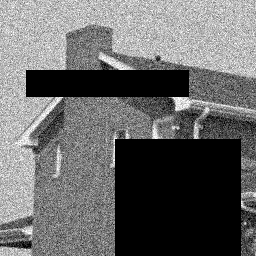
\includegraphics[width=0.25\textwidth]{fig/houseM-input.png}
    }
    \subfloat[ICM]{ \label{fig:eq:gm_ef_dension_icm}
        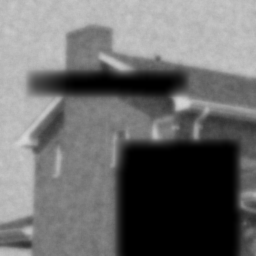
\includegraphics[width=0.25\textwidth]{fig/houseM-ICM.png}
    }
    \subfloat[$\alpha$-Expansion]{  \label{fig:eq:gm_ef_dension_ae}
        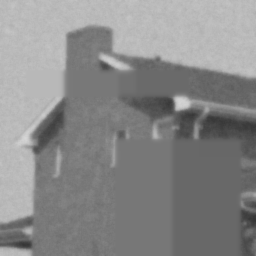
\includegraphics[width=0.25\textwidth]{fig/houseM-Expansion.png}
    }
    \subfloat[TRWS]{  \label{fig:eq:gm_ef_dension_trws}
        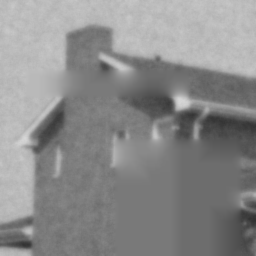
\includegraphics[width=0.25\textwidth]{fig/houseM-TRW-S.png}
    }
    \caption[Energy based truncated denoising]{
        Finding $x_{\text{optimal}} $ for the energy function given
        in \cref{eq:gm_ef_dension} is NP hard, we show result of approximative solvers.
        Using \cref{fig:eq:gm_ef_dension_input} as input (for the black area no unaries 
        are used)
        the following
        results are obtained:
        ICM
         \citep{besag_1986_icm}  (\Cref{fig:eq:gm_ef_dension_icm} ) fails
        to fill the in-painting area. 
        While TRWS
        \citep{kolmogorov_2006_pami_trws}  (\Cref{fig:eq:gm_ef_dension_trws} ) 
        and $\alpha$-Expansion
        \citep{boykov_2001_pami}  (\Cref{fig:eq:gm_ef_dension_ae} ) 
        can fill the in-painting area
        with meaningful values.
        The input image has been taken from \citep{szeliski_2008_pami}.
        The result images have been generated with OpenGM.
    }\label{fig:gm_ef_denoise}
\end{figure}

This model has been proposed by \citep{szeliski_2008_pami} where they proposed a MRF-benchmark.


\paragraph{Truncated Denoising:} 

This model is almost the same as the \emph{Denoising} model defined above,
but the second order term is truncate to $\gamma$ if $(x_i-x_j)^2$ is larger than $\gamma$.
Therefore we do pay only $\gamma$ at strong edges.
This model has also been proposed by \citep{szeliski_2008_pami} within their MRF-benchmark.


\begin{equation} \label{eq:gm_ef_dension_truncated}
E(x) = \sum_{v \in V}  (I_i - x_i)^2 + \sum_{e=(i,j) \in E } \lambda \cdot \min\left( (x_i-x_j)^2, \gamma\right)
\end{equation}

\begin{figure}[H]
    \centering
    \subfloat[Input Image $I$]{ \label{fig:eq:gm_ef_dension_truncated_input}
        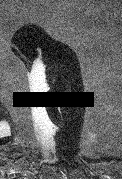
\includegraphics[width=0.25\textwidth]{fig/penguin-bar.png}
    }
    \subfloat[ICM]{ \label{fig:eq:gm_ef_dension_truncated_icm}
        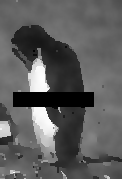
\includegraphics[width=0.25\textwidth]{fig/penguin-ICM.png}
    }
    \subfloat[$\alpha$-Expansion]{  \label{fig:eq:gm_ef_dension_truncated_ae}
        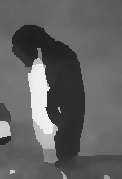
\includegraphics[width=0.25\textwidth]{fig/penguin-Expansion.png}
    }
    \subfloat[Trws]{  \label{fig:eq:gm_ef_dension_truncated_trws}
        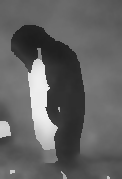
\includegraphics[width=0.25\textwidth]{fig/penguin-TRW-S.png}
    }
    \caption[Energy based truncated denoising]{
        Finding $x_{\text{optimal}} $ for the energy function given
        in \cref{eq:gm_ef_dension_truncated} we show result of approximative solvers.
        Using \cref{fig:eq:gm_ef_dension_truncated_input} as input (for the black area no unaries 
        are used)
        the following
        results are obtained: ICM \citep{besag_1986_icm}  (\Cref{fig:eq:gm_ef_dension_truncated_icm} ) fails
        to fill the in-painting area. While TRWS \cite{kolmogorov_2006_pami_trws}  (\Cref{fig:eq:gm_ef_dension_truncated_trws} ) 
        and $\alpha$-expansion \cite{boykov_2001_pami}  (\Cref{fig:eq:gm_ef_dension_truncated_ae} ) can fill the in-painting area
        with meaningful values.
        The input image has been taken from \citep{szeliski_2008_pami}.
        The result images have been generated with OpenGM.
        In contrast to the result of \cref{eq:gm_ef_dension}, this model
        allows sharp edges.
    }\label{fig:gm_ef_dension_truncated}
\end{figure}


\paragraph{Ferromagnetic Ising model}
The ferromagnetic ising model consists 
of binary variables.
The unaries encode local costs for a variable
to take label $0$ or $1$.
The pairwise term is a smoothness prior, which penalizes
adjacent variables with different states.

\begin{equation} \label{eq:gm_ising}
    E(x) = 
    \underbrace{
        \sum_{v \in V} \phi_i(x_i)
    }_{\text{unaries}}
     \quad +  \quad
    \underbrace{
        \beta \cdot \sum_{e=(i,j) \in E }  \delta(\cdot x_i\neq x_j) 
    }_{\text{pairwise potts terms}}
\end{equation}
Where $\detla(a)=1$ if $a$ is true and $0$ else
and $\beta>0$.
A large value of $\beta$

This model is also known as potts model and is often
used for binary segmentation (\eg foreground background segmentation).


\begin{figure}[H]
    \centering
    \subfloat[Input Image $I$]{ \label{fig:eq:gm_ef_ising_input}
        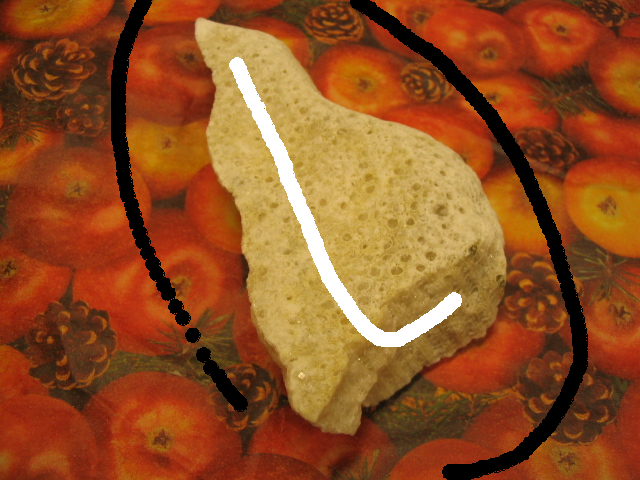
\includegraphics[width=0.25\textwidth]{fig/sponge.png}
    }
    \subfloat[ICM]{ \label{fig:eq:gm_ef_ising_icm}
        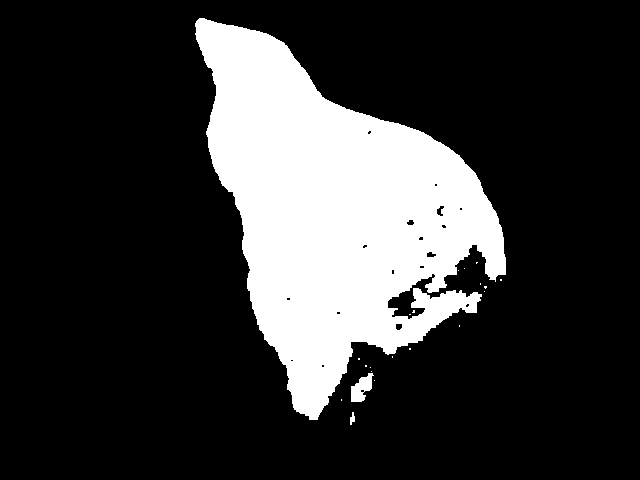
\includegraphics[width=0.25\textwidth]{fig/s_icm.png}
    }
    \subfloat[BP]{  \label{fig:eq:gm_ef_ising_bp}
        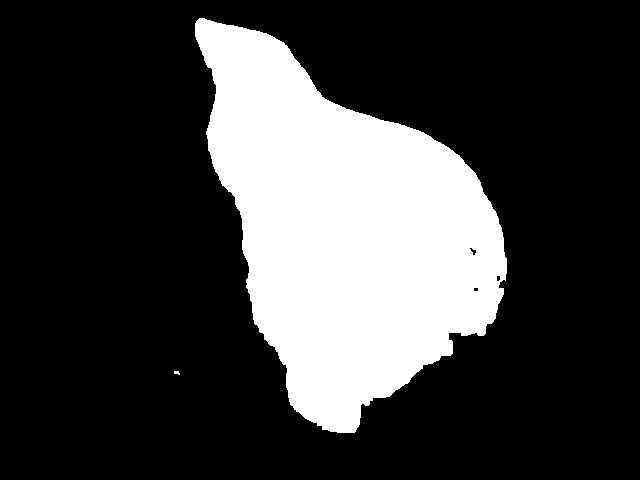
\includegraphics[width=0.25\textwidth]{fig/s_bp.png}
    }
    \subfloat[Graph Cut]{  \label{fig:eq:gm_ef_ising_cg}
        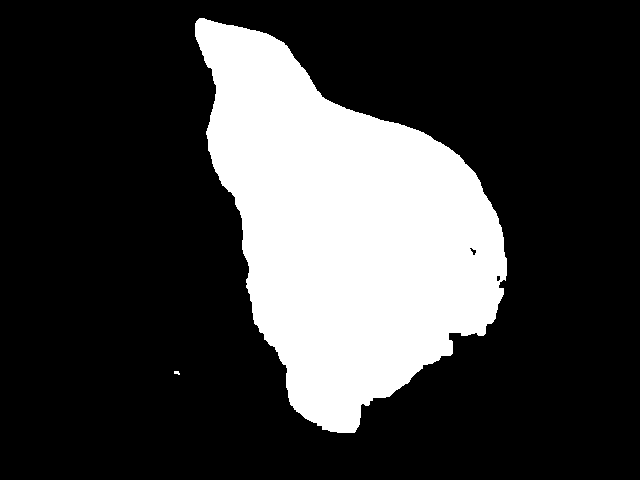
\includegraphics[width=0.25\textwidth]{fig/s_gc.png}
    }
    \caption[Potts Model]{
        Optimization results for the model defined in \cref{eq:gm_ising}.
        \Cref{fig:eq:gm_ef_ising_input} shows the input image.
        The unaries are based on a Gaussian mixture color models of foreground and background seeds defined by the user.
 
    }\label{fig:gm_ef_ising}
\end{figure}





\paragraph{Multicut Energy Function:}


Segmentation is an important problem in computer vision as a first step
towards understanding an image. Many algorithms start with an over-segmentation
into superpixels, which are then clustered into ``perceptually meaningful''
regions.
Usually, the number of these regions is not known beforehand.

Recently, the multicut formulation~\cite{chopra_1993_mp} 
(sometimes called \emph{correlation clustering}, \cite{bansal_2004_ml}) 
has become increasingly popular for unsupervised
image segmentation \cite{andres_2011_iccv,yarkony_2012_eccv,alush_2013_simbad}.

In this section we will give a brief overview of methods using multicut objectives
and will briefly introduce the multicut formulation.
The multicut and related work will be discussed extensively in \cref{ch:cgc} where
we propose a new approximative solver for the such problems.


Given an edge-weighted region adjacency graph,
the problem is to find the segmentation which
minimizes the cost of the cut edges.
Therefore multicuts can be viewed as \emph{thresholding} w.r.t. close contours, while
naive thresholding will lead to inconsistencies 
(see \cref{fig:naive_thresholding,fig:mc_ineq} ).


\begin{figure}[h]
    \centering
    \subfloat[Oversegmentation]{ \label{fig:naive_thresholding_a}
        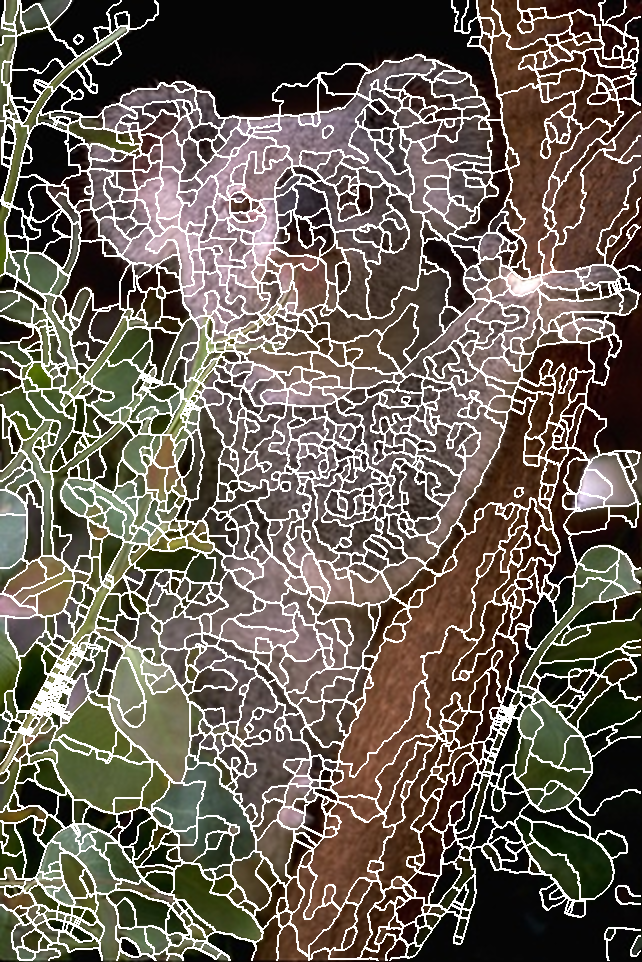
\includegraphics[width=0.25\textwidth]{fig/andres/0.png}
    }
    \subfloat[Oversegmentation]{  \label{fig:naive_thresholding_b}
        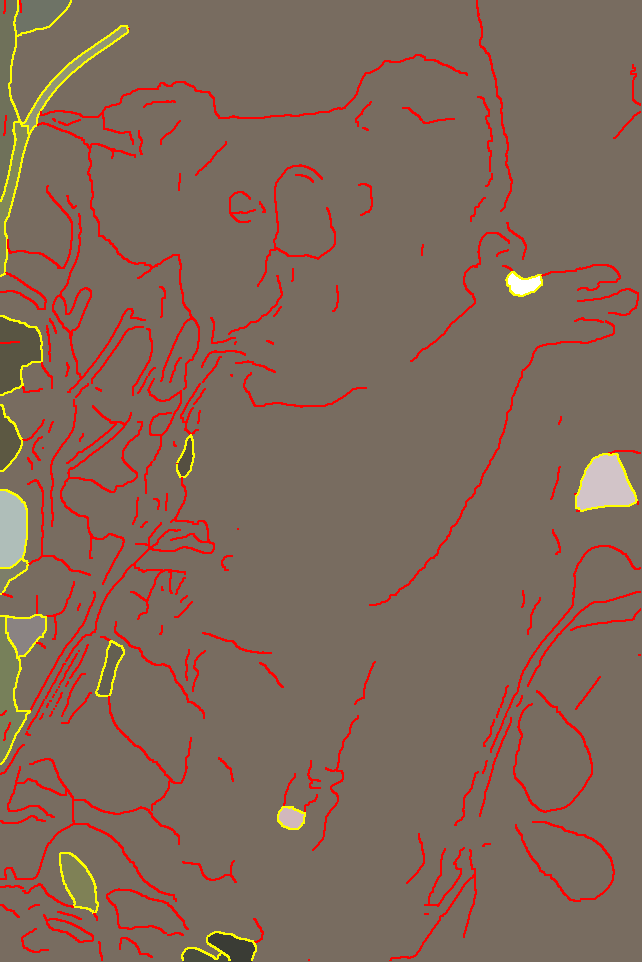
\includegraphics[width=0.25\textwidth]{fig/andres/1.png}
    }
    \subfloat[Oversegmentation]{  \label{fig:naive_thresholding_c}
        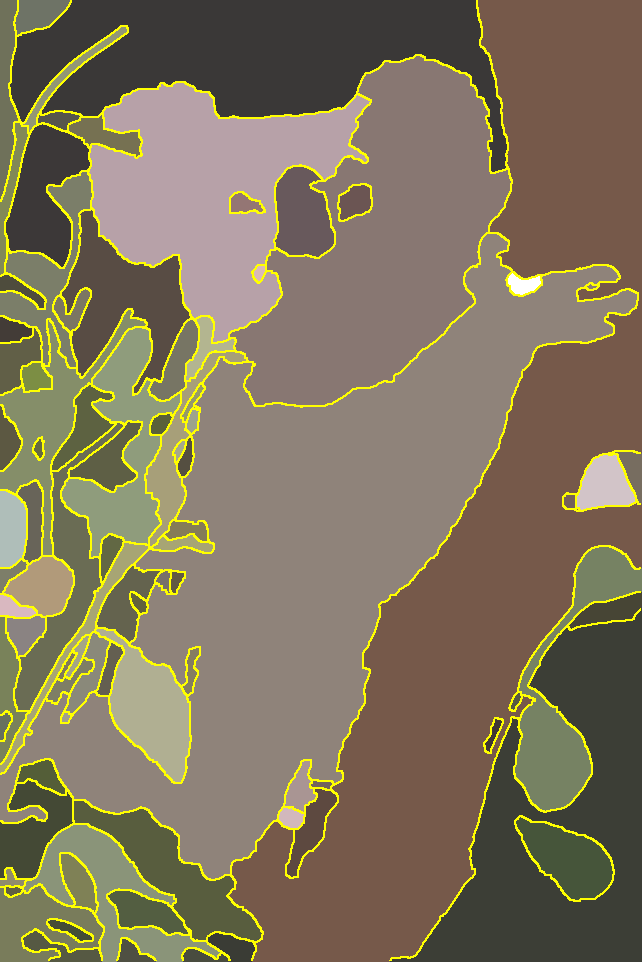
\includegraphics[width=0.25\textwidth]{fig/andres/2.png}
    }
    \addtocontents{lof}{%
        \vspace{1cm}
        \protect\centerline{%
            \protect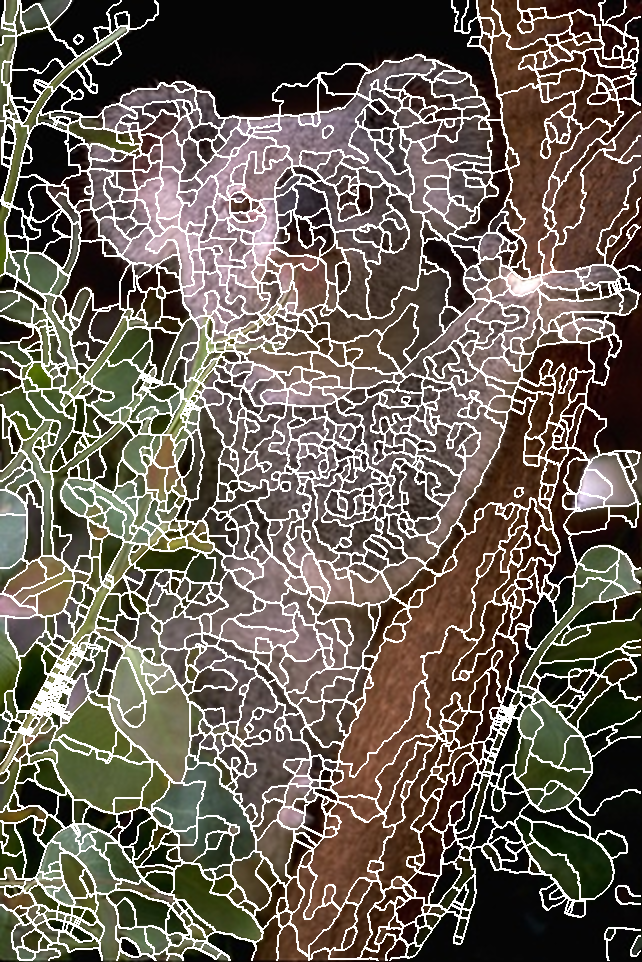
\includegraphics[width=.075\linewidth]{fig/andres/0.png}\hspace{0.2cm}
            \protect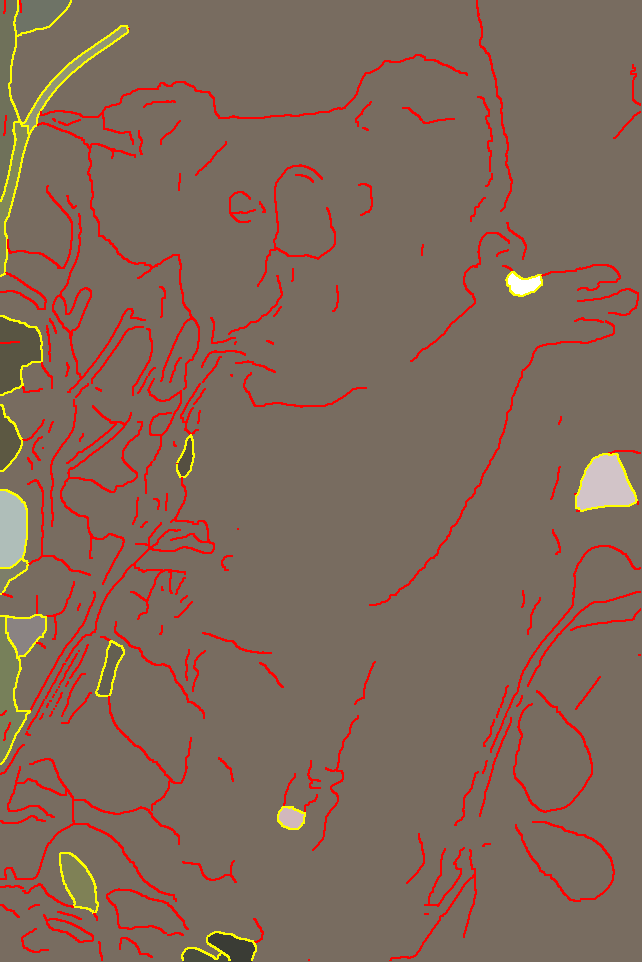
\includegraphics[width=.075\linewidth]{fig/andres/1.png}\hspace{0.2cm}
            \protect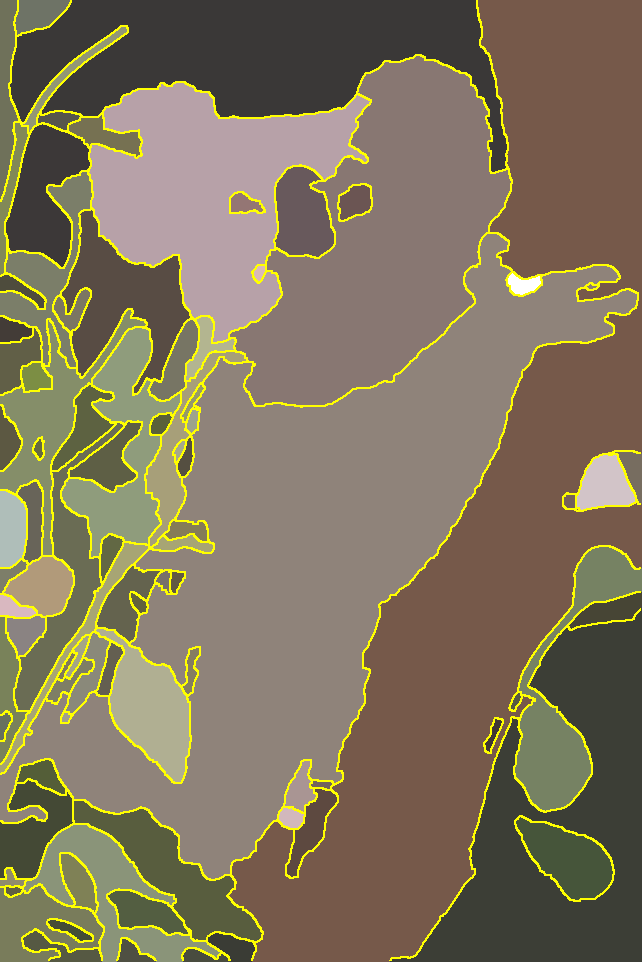
\includegraphics[width=.075\linewidth]{fig/andres/2.png} 
        }%
    }%
    \caption[Naive thresholding vs. multicuts]{
    This figure has been taken from \cite{andres_2011_iccv} .
    \Cref{fig:naive_thresholding_a} shows the oversegmentation of 
    an image .
    \Cref{fig:naive_thresholding_b} shows the result of naive thresholding..
    Any inconsistent boundary is shown in red while consistent
    boundaries are shown in yellow. 
    \Cref{fig:naive_thresholding_c} shows the result with the multicut
    constraints which lead to a meaningful segmentation.
    } \label{fig:naive_thresholding}
\end{figure}



Let $G=(V,E, \w)$ be a weighted region adjacency graph of
nodes $V$, representing superpixels,
and edges $E$.
%
The function $\w : E \rightarrow \mathbb{R}$ assigns a weight to each edge.
A positive weight expresses the desire that two adjacent nodes should
be merged, whereas a negative weight indicates
that these nodes should be separated into two different regions.


The \emph{multicut problem} can be written as a node labeling problem
\cite{bagon_2011_arxiv}:
%
\begin{align}
\argmin_{\Labels}
    \left\{
    \sum_{ e=(i,j) \in E}
        \w(e)
        \cdot \delta( \Labels_i \neq \Labels_j )
    \right\},
    \label{eq:multicut_primal_a}
\end{align}
%
where $\delta(a) = 1$ if $a$ is true and $0$ else.


Removing all unaries from \cref{eq:gm_energy} and 
setting $\phi_{ij}(x_i,x_j) =   \w_e \cdot \delta( x_i \neq x_j )$ 
will lead to the multicut objective (see \cref{ch:cgc}) .

For planar problems  $N_{labels}$ can be set to 4 since any planar map is 4 colorable \citep{appel_1977_4color}.
For non planar problems we need to set $N_{labels}$ to $|V|$.


\citet{andres_2011_iccv} and \citet{kappes_2011_emmcvpr} use a
cutting plane approach where violated constraints are added
iteratively until no more violated constraints are found.

\begin{figure}[h]
\centering
\subfloat[Superpixel Segmentation]{ \label{fig:mc_ineq_0}
    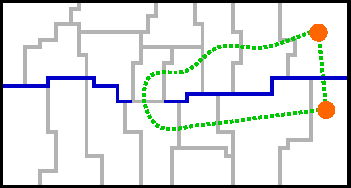
\includegraphics[width=0.4\textwidth]{fig/andres/ineq_0.pdf}
}
\subfloat[Corresponding Graph]{ \label{fig:mc_ineq_1}
    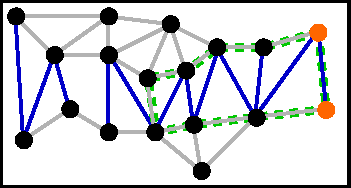
\includegraphics[width=0.4\textwidth]{fig/andres/ineq_1.pdf}
}
\addtocontents{lof}{%
    \vspace{1cm}
    \protect\centerline{%
        \protect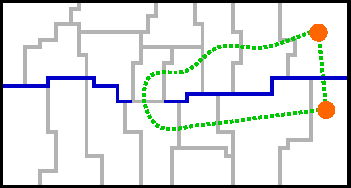
\includegraphics[width=.075\linewidth]{fig/andres/ineq_0.pdf}\hspace{0.2cm}
        \protect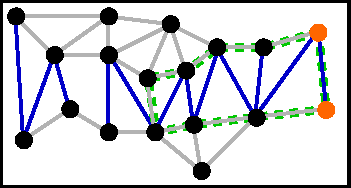
\includegraphics[width=.075\linewidth]{fig/andres/ineq_1.pdf}
    }%
}%
\caption[Violated multicut constraints]{
This figure has been taken from \cite{andres_2011_iccv}.



\Cref{fig:mc_ineq_0} shows the oversegmentation of 
an image .
\Cref{fig:mc_ineq_1} shows the corresponding graph.
Thresholding each edge individually will lead to inconsistencies.
The current state of the edges  labeled as active (blue) or inactive (gray) is
inconsistent: Some nodes should be separated, since the edge between them is
active (blue), but there exists a path over inactive edges 
which connects these two nodes (showed in green).
} \label{fig:mc_ineq}
\end{figure}


\begin{align}
E(x)=
    \sum_{ e=(i,j) \in E}
        \w_e \cdot \delta( x_i \neq x_j )
    \label{eq:gm_ef_multicut}
\end{align}


The \emph{max-cut} objective and  the multicut objective
are almost the same, 
but within max-cut problem we have only binary variable $x_i=\{0,1\}$ .

\begin{align}
E(x)=
    \sum_{ e=(i,j) \in E}
        \w_e \cdot \delta( x_i \neq x_j )
    \label{eq:gm_ef_max_cut}
\end{align}




\subsection{Graph Cut Based Methods}

If $N_{labels}=2$ and $\phi_{ij}(x_i,x_j)$ is submodular, 
graph cuts \cite{boykov_2001_pami,kolmogorov_2004_pami} can be applied to find $x_{\text{optimal}}$
in polynomial time.

Graph cut is a optimization algorithm which casts the energy minimizing problem
to the maximum flow / minimum cut problem. Energy function of binary variables which
have a form as 

\begin{equation} \label{eq:gm_graph_cut_energy}
    E(x) = 
    \underbrace{
        \sum_{v \in V} \phi_i(x_i)
    }_{\text{unaries}}
     \quad +  \quad
    \underbrace{
        \sum_{e=(i,j) \in E } \phi_{ij}(x_i,x_j) 
    }_{\text{submodular pairwise terms}}
\end{equation}



where the pairwise energy term of binary variables is submodular can be minimized with
graph cuts. $\phi_{ij}$ is submodular if

\begin{equation} \label{eq:gm_submodular_criterion}
    \phi_{ij}(0,1) + \phi_{ij}(1,0) >  \phi_{ij}(0,0) + \phi_{ij}(1,1)
\end{equation}

To use graph cut, we have to associate each possible solution with a cut on a graph as in
\cref{fig:graph_cut} and ensure that the capacities on the graph match our energy function 
defined in \cref{eq:gm_graph_cut_energy}.
Since the max flow/ min cut problem is defined on a directed graph, we have to construct
a directed graph from the energy function we want to minimize. We add a source and a
sink vertex and connect these terminal vertices with all variable vertices and assign
each edge a non-negative flow capacity. The flow goes from the source vertex to the
sink vertex. The edge capacities are constructed as described in the work of
\citet{kolmogorov_2004_pami}.

\Cref{fig:graph_cut_b} shows how the
construction of the directed weighted graph which associate with the energy function $E(x)$.
\citet{kohli_2007_pami} proposed a method to change some and resolve
the problem efficiently which allows a fast computation
of graph cut min marginal an uncertainties \citep{kohli_2006_eccv,tarlow_2012_cvpr}.


\begin{figure}[H]
\begin{center}
\subfloat[$ $]{\label{fig:graph_cut_a}
    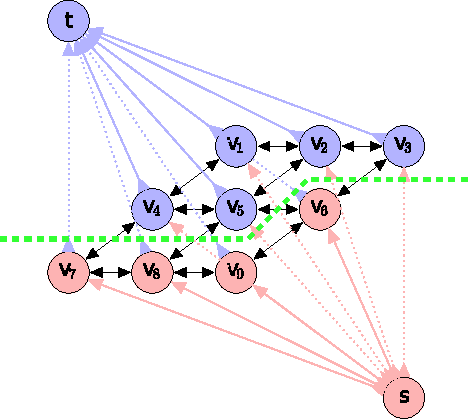
\includegraphics[height=0.3\textwidth]{fig/min_st.pdf}   
}
\hspace{1.5cm}
\subfloat[$ $]{\label{fig:graph_cut_b}
    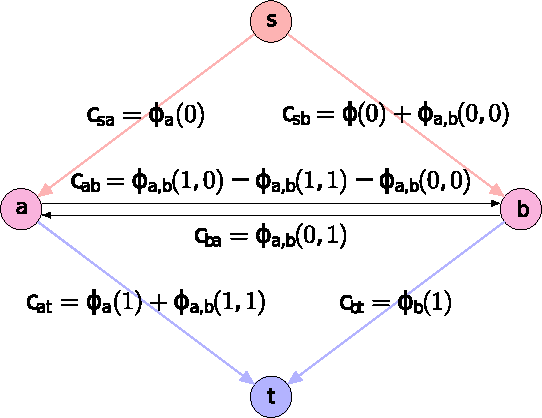
\includegraphics[height=0.3\textwidth]{fig/min_st_d.pdf}   
}
\end{center}
\caption{
    \Cref{fig:graph_cut_a}: Each variable vertex is connected to the 2 terminal vertices, source s, and
        sink t, the edges between the variables vertices and terminal vertices are
        called t-links, the edges between variables vertices are called n-links. The
        line dotted in green is a cut, separating the variable with state zero from
        those with state one.
    \Cref{fig:graph_cut_b} is a simplification of the construction of the weighted graph.
        A constant term $\beta$ which has to be added to some capacities
        has been omitted for simplicity. 
        Interested readers are refereed to  the work of \citet{kolmogorov_2004_pami}.
}\label{fig:graph_cut}
\end{figure}


Whenever we have a a energy function of binary variables with pairwise potentials which
are non-submodular we cannot use graph cut. QPBO (quadratic pseudo-boolean optimization), 
the work of \citet{rother_2007_cvpr}, 
addresses the problem of minimizing such an energy function as the
following:

\begin{equation} \label{eq:gm_qpbo_energy}
    E(x) = 
    \underbrace{
        \sum_{v \in V} \phi_i(x_i)
    }_{\text{unaries}}
    \quad +  \quad
    \underbrace{
        \sum_{e=(i,j) \in E } \phi^{s}_{ij}(x_i,x_j)
    }_{\text{submodular pairwise terms}}
    \quad +  \quad
    \underbrace{
        \sum_{e=(i,j) \in E } \phi^{\bar{s}}_{ij}(x_i,x_j)
    }_{\text{non-submodular pairwise terms}}
\end{equation}

The basic idea of QPBO is to relax the problem by optimizing an auxiliary graphical
model with twice as much variables as the problem we want to optimize. The
auxiliary problem is constructed in such a way that it is submodular. The
auxiliary problem is constructed as in \cite{rother_2007_cvpr} and optimized with graph cut. 
The output of QPBO
is a partial labeling $x_i \in \{ 0,1, EPT \}$. $EPT$ is interpreted as unknown state. There are several
extension to improve which reduce the number
of variables which have the state $EPT$ .


If the label space is larger than 2, $\alpha$-expansion and $\alpha \beta$-swap \cite{boykov_2001_pami} can be used.
The main idea of $\alpha$-expansionm is to iteratively
solve binary sub-problems, where one only has to decide whether a variable should be
flipped to the state $\alpha$ or keep the current state. The value of $\alpha$ is changed in each iteration.

$\alpha \beta$-swap] is very similar  $\alpha$-expansion.
But this time we have two labels, $\alpha$ and $\beta$. Within each iteration variables
with the state $\alpha$ can be flipped to the state $\beta$ and visa versa. The values of $\alpha$ and $\beta$
are changed after each iteration.

If the binary sub-problems are submodular graph cut can be used, otherwise QPBO.



\subsection{Linear Programming Methods}



An alternative formulation of the multicut objective \cref{eq:multicut_primal,eq:gm_ef_multicut} 
is in terms of binary edge indicator variables.
$\y \in \{0,1\}^{| E |}$:
\begin{align}
\argmin_{\y}
%
\left\{
    \sum_{e=(i,j) \in E} \w \left(e\right) \cdot \y_{e}
\right\}%
%
\;\;\text{s.t.}\;\;\y \in \MC_G.
\label{eq:multicut_dual_a}
\end{align}
%
%
$\text{MC}_G$ is the set of all multicut
constraints \cite{chopra_1993_mp} for graph $G$ forming
the so called \emph{multicut polytope}.
The objective in \cref{eq:multicut_dual_a}
is linear w.r.t. indicator variables $\y_{e}$.

In general,
$\y \in \MC_G$ can be enforced by an exponential number of
constraints \cite{chopra_1993_mp}, but in practice
-- for a given objective function --
a small subset of those are sufficient.
Therefore, a major branch of research has focused 
on cutting plane approaches,
either by solving a relaxation of \eqref{eq:multicut_dual}
by a sequence of linear programs 
\cite{kim_2011_nips,kim_2012_ip,kappes_2013_arxiv,finley_2005_ml}.














To apply linear programming methods to minimize a general discrete energy function, 
the energy functions
needs to be linearized.

To optimize an energy functions as 

\begin{equation} \label{eq:gm_nl_energy}
    E(x) = 
     \sum_{v \in V}
    \underbrace{
        \phi_i(x_i)
    }_{\text{unaries}}
     \quad +  \quad
     \sum_{e=(i,j) \in E } 
    \underbrace{
        \phi_{ij}(x_i,x_j) 
    }_{\text{pairwise terms}}
\end{equation}

we introduce $\mu_{i}^{l}$ as an indicator variable where $\mu_{i}^{l}=1$ indicates $x_i=l$.
In the same manner we use $\mu_{ij}^{l_a l_b}$ to indicate pairwise 
assignments.
The constraints ensure that the indicator variables $\mu_{i}^{l}$ are consistent 
with pairwise indicators $\mu_{ij}^{l_a l_b}$ .

The set of these consistency constraints is 
called \emph{local consistency constraints} \citep{sontag_2010_thesis}.

\begin{align}
    E(\mu) = \sum_{v \in V} \sum_{l=0}^{L_{\text{max}}} \label{eq:gm_lp}
    \mu_{i}^{l} \cdot \phi_{i}( l)
    \quad +  \quad
    %
    \sum_{e \in E} \sum_{l_a=0}^{L_{\text{max}}} \sum_{l_b=0}^{L_{\text{max}}}
    \mu_{ij}^{l_a l_b} \cdot \phi_{ij}( l_a,l_b) \\
    %
    s.t. \quad
    \sum_{l=0}^{L_{\text{max}}} \mu_{i}^{l} = 1 \quad \forall \quad v_i \in V \\
    %
    \sum_{l_b=0}^{L_{\text{max}}} \mu_{ij}^{l_a l_b} = \mu_i 
    \quad \forall \quad e_{ij} \in E, 
    \quad l_a \in \{ 0,1,\ldots,L_{\text{max}} \} \\ 
    %
    \sum_{l_a=0}^{L_{\text{max}}} \mu_{ij}^{l_a l_b} = \mu_j 
    \quad \forall \quad e_{ij} \in E, 
    \quad l_b \in \{ 0,1,\ldots,L_{\text{max}} \} \\ 
    %
    \mu_i^l \geq 0 \quad \forall \quad v_{i} \in V,
    \quad l \in \{ 0,1,\ldots,L_{\text{max}} \}\\
    \mu_{ij}^{l_a l_b} \geq 0 \quad \forall \quad e_{ij} \in E,
    \quad l_a,l_b \in \{ 0,1,\ldots,L_{\text{max}} \}
\end{align}

Solving the LP in \cref{eq:gm_lp} will lead to fractional
solutions since the \emph{local consistency constraints} 
define a polytope which is a relaxation
of the marginal polytope.
In \cref{fig:local_poly} is a visualization of the local
polytope \footnote{
Interested readers are refereed to the doctoral
thesis of  \citet{sontag_2010_thesis} which gives
a great overview and introduction to linear programming
based optimization.
}.

An additional set of constraints, \emph{integer constraint} can be added the LP in \cref{eq:gm_lp}. These constraints turn the LP into an integer LP (I-LP).

\begin{align}
    \mu_i^l \in \{0,1\} \quad \forall \quad v_{i} \in V,
    \quad l \in \{ 0,1,\ldots,L_{\text{max}} \} \label{eq:integral_constraint}
\end{align}

Solving the I-LP yields
global optimal solutions of the energy function defined in 
\cref{eq:gm_nl_energy}.







\begin{figure}[H]
\centering
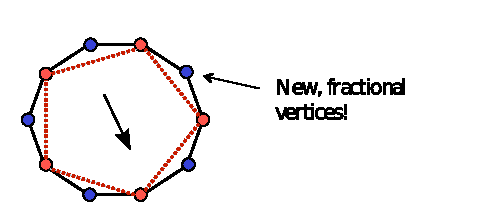
\includegraphics[width=0.6\textwidth]{fig/frac_vert2.pdf}
\caption{
    A sketch of the local consistency polytope.
    The local polytope is a relaxation
    of the marginal polytope (red dashed lines).
    While the marginal polytope has only integral
    nodes (red nodes , the local polytope 
    will introduce fractional vertices which are shown
    in blue.
    The figure has been taken from \citep{sontag_2010_thesis}
    an has been modified slightly.
    Interested readers are refereed to the doctoral
    thesis of  \citet{sontag_2010_thesis} which gives
    a great overview and introduction to linear programming
    based optimization.
}\label{fig:local_poly}
\end{figure}





